\documentclass[border=4pt]{standalone}
\usepackage{tikz}
\usetikzlibrary{arrows.meta,positioning,fit,backgrounds,calc,shapes.geometric}
\definecolor{snblue}{HTML}{1F5A96}
\definecolor{snred}{HTML}{B8433A}
\definecolor{sngreen}{HTML}{3A8A4A}
\tikzset{
  pb/.style={rectangle,rounded corners=3pt,draw=snblue!60,fill=snblue!8,text width=2.3cm,align=center,inner sep=4pt,line width=0.5pt,font=\small},
  db/.style={pb,draw=snred!55,fill=snred!6},
  gb/.style={pb,draw=sngreen!60,fill=sngreen!8},
  dm/.style={diamond,aspect=2.2,draw=gray!70,fill=gray!6,align=center,inner sep=1pt,font=\small},
  ar/.style={-Stealth,line width=0.6pt,gray!70}}

\begin{document}
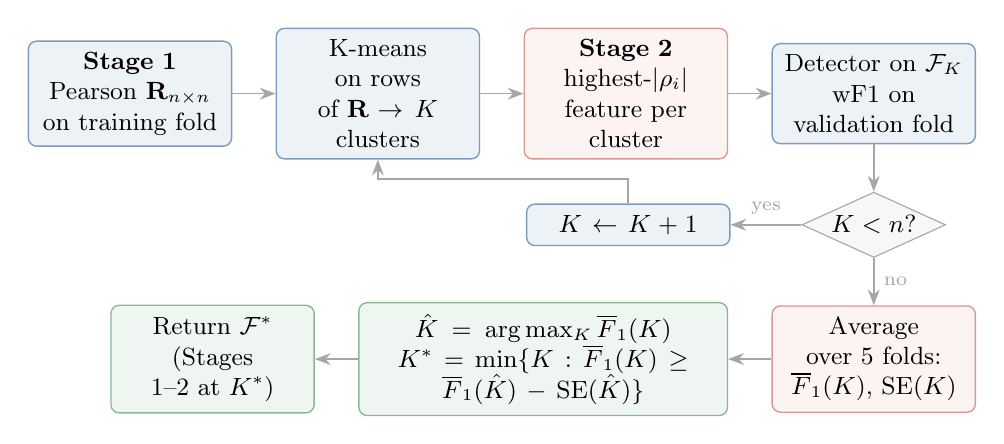
\begin{tikzpicture}[node distance=0.45cm and 0.55cm]
\node[pb](r){\textbf{Stage 1}\\Pearson $\mathbf{R}_{n\times n}$\\on training fold};
\node[pb,right=of r](km){K-means on rows\\of $\mathbf{R}$ $\to K$ clusters};
\node[db,right=of km](rk){\textbf{Stage 2}\\highest-$|\rho_i|$\\feature per cluster};
\node[pb,right=of rk](ev){Detector on $\mathcal{F}_K$\\wF1 on validation fold};
\node[dm,below=0.6cm of ev](more){$K<n$?};
\node[pb,left=0.9cm of more](inc){$K\gets K+1$};
\node[db,below=0.6cm of more](agg){Average over 5 folds:\\$\overline{F}_1(K)$, $\mathrm{SE}(K)$};
\node[gb,left=of agg,text width=4.4cm](rule){$\hat K=\arg\max_K\overline{F}_1(K)$\\$K^{*}=\min\{K:\overline{F}_1(K)\ge\overline{F}_1(\hat K)-\mathrm{SE}(\hat K)\}$};
\node[gb,left=of rule](out){Return $\mathcal{F}^{*}$\\(Stages 1--2 at $K^{*}$)};
\draw[ar](r)--(km);\draw[ar](km)--(rk);\draw[ar](rk)--(ev);\draw[ar](ev)--(more);
\draw[ar](more)--node[above,font=\scriptsize]{yes}(inc);
\draw[ar](inc.north)|-([yshift=-0.25cm]km.south)--(km.south);
\draw[ar](more)--node[right,font=\scriptsize]{no}(agg);
\draw[ar](agg)--(rule);\draw[ar](rule)--(out);
\end{tikzpicture}
\end{document}
